We can draw box-and-pointer diagrams to help us visualize Scheme pairs and
lists.

A pair is represented as two boxes, each containing one element of the pair.
For example, to draw the pair constructed by \texttt{(cons 1 nil)}: \\

\includegraphics[scale=.7]{../topics/scheme/images/pair.png}

To draw lists, draw a series of pairs connected by arrows.
Specifically, the first item in each pair corresponds to an item in the list.
The second item in each pair is an arrow to the rest of the list. Here is the
list \texttt{(1 2 3)}: \\
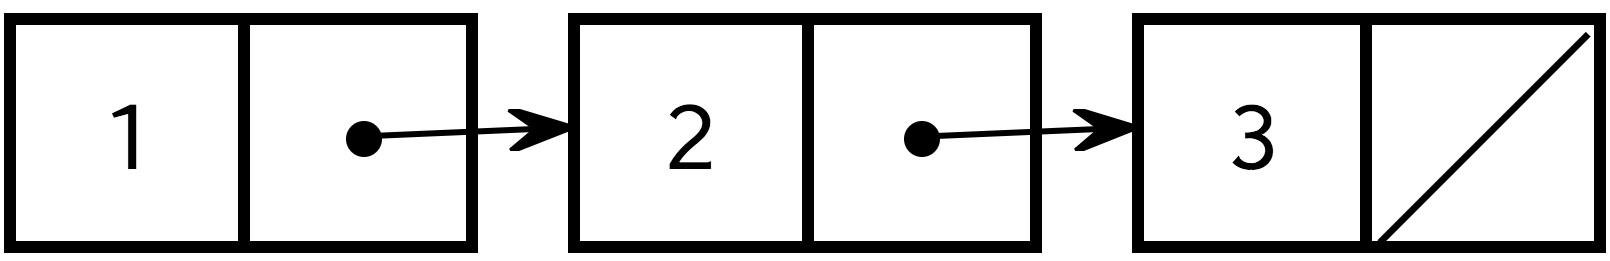
\includegraphics[scale=0.25]{../topics/scheme/images/list123.png}
